\documentclass[11pt,a4paper]{article}
\usepackage{amsmath}
\usepackage{amssymb}
\usepackage{amsthm}
\usepackage[utf8]{inputenc}
\usepackage{graphicx}

\usepackage[utf8]{inputenc}
\usepackage[english]{babel}
 
\usepackage{cite}


\newtheorem{theorem}{Theorem}

\usepackage{listings}
\usepackage{color} %red, green, blue, yellow, cyan, magenta, black, white
\definecolor{mygreen}{RGB}{28,172,0} % color values Red, Green, Blue
\definecolor{mylilas}{RGB}{170,55,241}


\usepackage{graphicx}

\title{Optimal control with DE constraints}



\begin{document}
\maketitle
\tableofcontents
\section{Literature}
In the paper \cite{maday2002parareal}, Maday and Turinici presents a way to solve a control problem with partial differential evolution constraints in parallel using parareal. The problem they look at is the following:
\begin{align*}
J(y,u) = \frac{1}{2}\int_0^T||u(t)||_U^2dt + \frac{\alpha}{2}||y(T)-y^T||^2
\end{align*} 
For the equation:
\begin{align*}
\left\{
     \begin{array}{lr}
       	\frac{\partial y}{\partial t}+Ay = Bu\\
       	   y(0)=y_0
     \end{array}
   \right.
\end{align*}
They parallelize in time, by dividing up the time interval and enforcing continuity by adding a penalty to the functional. They then derive the adjoint equation and the gradient for the functional. The idea of parareal, is to sequentially solve a differential equation on a coarser mesh, and then using this solution to solve the same equation in parallel. This approach is necessary to get a speed-up for the virtual problem(i.e. just solving the equation), but the coarse sequential solve also represents a bottleneck for scalability. This is addressed in \cite{rao2014adjoint}, where they try to parallelize PDEs in time in a scalable way, by only doing an initial coarse sequential solve, and thereafter doing everything in parallel.  
\\
\\
In \cite{rao2016time} the authors propose a augmented Lagrangian approach for time-parallel 4d variational data assimilation. This is basically a optimal control problem with PDE constraints. The augmented Lagrangian method is a modification of the penalty method for unconstrained optimization. Algorithms for calculating the modified functional and the gradient of the modified functional is derived, and the method is tested on a problem. The results show weak scalability for gradient and functional evaluation.  
\section{General Problem}
Looking at an optimal control problem $$\underset{y,u}{\text{min}} \ J(y,u) \ \text{subject to} \ E(y,u)=0$$ Where $u \in U$ is the control and $y \in Y$ is the state that depends on $u$. Usually $u$ and $y$ are functions, and $U$ and $Y$ are either Hilbert or Banach spaces. I will not go into detail about these spaces, but they are mostly chosen to fit the differential equation $E$, which is an operator on $U\times Y$.
\\
\\
Differentiating $J$ is required for solving the problem. To do this we reduce $J$ to $\hat{J}(u) = J(y(u),u) $ and compute its gradient in direction $s \in U$. Will use the notation: $\langle\hat{J}'(u),s\rangle$ for the gradient.
\begin{align*}    
\langle\hat{J}'(u),s\rangle &= \langle DJ(y(u),u) ,s\rangle \\ &= \langle \frac{\partial y(u)}{\partial u}^*J_y(y(u),u),s\rangle + \langle J_u(y(u),u),s\rangle \\ &= \langle y'(u)^*J_y(u),s\rangle +\langle J_u(u),s\rangle
\end{align*}
Here $\langle\cdot,\cdot\rangle$ is the $U$ inner product. The difficult term in the expression above is $y'(u)^*$, so lets first differentiate $E(y(u),u)=0$ with respect to $u$, and try to find an expression for $y'(u)^*$: 
\begin{align*}
\frac{\partial}{\partial u}E(y(u),u)=0 &\Rightarrow E_y(y(u),u)y'(u)=-E_u(y(u),u) \\ &\Rightarrow y'(u)=-E_y(y(u),u)^{-1}E_u(y(u),u) \\ &\Rightarrow y'(u)^* = -E_u(y(u),u)^*E_y(y(u),u)^{-*}
\end{align*} 
By inserting our new expression for $y'(u)^*$ into $y'(u)^*J_y(u)$, we get:
\begin{align*}
y'(u)^*J_y(u)&=-E_u(y(u),u)^*E_y(y(u),u)^{-*}J_y(u) \\
&=-E_u(y(u),u)^*p
\end{align*}
p is here the solution of the adjoint equation 
\begin{gather*}
E_y(y(u),u)^{*}p=J_y(u)
\end{gather*}
If we can solve this equation for p, the gradient of $\hat{J}$ will be given by the following formula:  
\begin{gather}
\langle\hat{J}'(u),s\rangle=\langle -E_u(y(u),u)p,s\rangle +\langle J_u(u),s\rangle
\end{gather} 
\\
\\
\section{Optimal control with ODE constraints}
Lets try to derive the adjoint equation and the gradient, when we let $E(y,u)$ be the following ODE:
\begin{align*}
\left\{
     \begin{array}{lr}
       	y'(t)=\alpha y(t) +u(t), \ t \in (0,T)\\
       	   y(0)=y_0
     \end{array}
   \right.
\end{align*}
We also choose the functional to be
\begin{align*}
J(y,u) = \frac{1}{2}\int_0^Tu(t)^2dt + \frac{1}{2}(y(T)-y^T)^2
\end{align*}
Before we calculate the different terms in the gradient, we want to fit our ODE into an expression $E$. we do this by "moving" the initial condition into the equation:
\begin{align*}
E(y,u) = y'-\alpha y - u + \delta_0(y-y_0)
\end{align*}
Here the $\delta_0$ means evaluation at $0$. Now  lets find $E_u$, $E_y$, $ \langle J_u(u),s\rangle$ and $J_y$ with respect to our $E$ and $J$.
\begin{align*}
E_u(y(u),u)&=-1 \\
E_y(y(u),u)&=\frac{\partial}{\partial t} - \alpha + \delta_0 \ \text{,where $\delta_0$ is evaluation at 0} \\
\langle J_u(u),s\rangle &= \int_0^T u(t)s(t) dt 
\end{align*}
Lets be more thorough with $J_y$, which is the right hand side in the adjoint equation.
\begin{align*}
J_y(y(u),u) &= \frac{\partial}{\partial y}(\frac{1}{2}\int_0^Tu^2dt + \frac{1}{2}(y(T)-y^T)^2) \\ &= \frac{\partial}{\partial y} \frac{1}{2}(y(T)-y^T)^2 \\
&= \frac{\partial}{\partial y}\frac{1}{2}(\int_0^T \delta_T(y-y^T)dt)^2 \\
&= \delta_T\int_0^T \delta_T(y(t)-y^T)dt \\
&= \delta_T(y(T)-y^T)=L
\end{align*}
We have $E_y(y(u),u)=\frac{\partial}{\partial t} - \alpha + \delta_0$, but for the adjoint equation we need to find $E_y^*$.
To derive the adjoint of $E_y$, we will apply it to a function $v$ and then take the $L^2$ inner product with another function $w$. The next step is then to try to "move" the operator $E_y$ from $v$ to $w$. As becomes clear below, partial integration is the main trick to achieve this: 
\begin{align*}
\langle E_yv,w \rangle &=  \int_0^T(v'(t)-\alpha v(t)+\delta_0v(t))w(t)dt \\ &= \int_0^Tv'(t)w(t)dt -\alpha\int_0^Tv(t)w(t) dt +v(0)w(0) \\
& = -\int_0^Tv(t)w'(t)dt +v(t)w(t)|_0^T-\alpha\langle v,w\rangle +v(0)w(0) \\
&=-\int_0^Tv(t)w'(t)dt -\alpha\langle v,w\rangle +v(T)w(T) \\
&= \langle v,Pw \rangle
\end{align*} 
Where $P=-\frac{\partial}{\partial t} -\alpha + \delta_T$. This means that $E_y^* = P$, and we now have the left hand side in the adjoint equation. The right hand side is $J_y(y(u),u)=L$, which we have already found. If we write the  adjoint equation on variational form it will look like this: $\langle Pp,w\rangle = \langle L,w\rangle$. To get back to standard ODE form, we can do some manipulation: 
\begin{align*}
\langle -p'-\alpha p +\delta_T p,w \rangle &= \langle \delta_T(y(T)-y^T),w\rangle \\
\langle -p'-\alpha p ,w \rangle &= \langle \delta_T(y(T)-y^T -p),w\rangle
\end{align*}
The right hand side is point evaluation at $t=T$, while the left hand side is an expression for all $t$. This finally gives us our adjoint equation: 
\begin{align*}
   \left\{
     \begin{array}{lr}
       -p'(t) = \alpha p(t) \\
       p(T) = y(T)-y^T
     \end{array}
   \right.
\end{align*}
This is a simple and easily solvable ODE.
\\
\\
\textbf{Expression for the gradient}
\\
We now have all the ingredients for finding an expression for the gradient of $\hat{J}$. If we remember that $\langle\hat{J}'(u),s\rangle=\langle y'(u)^*J_y(u),s\rangle +\langle J_u(u),s\rangle$, and all the different expressions for all the terms we calculated, we find:
\begin{align*}
\langle\hat{J}'(u),s\rangle&=\langle y'(u)^*J_y(u),s\rangle +\langle J_u(u),s\rangle \\ &=\langle -E_u^*p,s\rangle +\langle J_u(u),s\rangle \\
&=\langle -(-1)^*p,s\rangle +\langle u,s\rangle \\
&=\langle p+u,s\rangle \\
&= \int_0^T(p(t)+u(t))s(t)dt
\end{align*} 
Note that the adjoint of a constant is just the constant itself.
\addcontentsline{toc}{section}{Parallelizeing in time using the penalty method}
\section*{Parallelizeing in time using the penalty method}
To find the above gradient, we must solve first the state equation forward in time and then the adjoint equation backwards in time. One way of speeding things up is to parallelize the solvers by partitioning the time interval and then solving the equation separately on each partitioned interval. If we split the interval $[0,T]$ into $m$ parts we need to solve $m$ state equations on the following form:
\begin{align*}
   \left\{
     \begin{array}{lr}
       \frac{\partial }{\partial t} y_i(t) = \alpha y_i(t) + u(t) \ \text{for $t \in [T_{i-1},T_{i}]$}\\
	y_i(T_{i-1}) = \lambda_{i-1}
     \end{array}
   \right.
\end{align*}
here $i=1,...,m$, $\lambda_0=y_0$ and $0=T_0<T_1<\cdots<T_{m}=T$. Since the equation on each interval depends on the equation in the previous interval, we need a trick, to get everything to hang together. We do this using the penalty method, which means adding a penalty to the functional. The new functional now looks like this:
\begin{align*}
J(y,u,\lambda) = \int_0^T u^2 dt + \frac{1}{2}(y_m(T)-y^T)^2 + \frac{\mu}{2} \sum_{i=1}^{m-1} (y_{i}(T_i)-\lambda_i)^2 
\end{align*}
This means that the problem now is to minimize $J$ with respect to both $u$ and $\lambda$, which means that the reduced functional depends on both $u$ and $\lambda$. Since we change the functional and the equation, both the adjoint equation and the gradient changes. Lets try to derive the new adjoint equations and the new gradient. The gradient of the reduced functional now looks like the following:
\begin{align*}
\langle \hat{J}'(u,\lambda), (s,l)\rangle &= \langle \frac{\partial y(u,\lambda)}{\partial(u,\lambda)}^* J_y(y(u,\lambda),u,\lambda), (s,l)\rangle + \langle J_u+J_{\lambda}, (s,l)\rangle \\
&=\langle -(E_u+E_{\lambda})p , (s,l)\rangle + \langle J_u+J_{\lambda}, (s,l)\rangle
\end{align*} 
Where p is the solution of the adjoint equation $E_y^*p=J_y$, and $E$ is our ODEs:
\begin{align*}
E^i(y,u,\lambda)= \frac{\partial }{\partial t} y_i - \alpha y_i -u+ \delta_{T_{i-1}}(y_i-\lambda_{i-1})
\end{align*} 
Lets differentiate $E$:
\begin{align*}
E_y^i &= \frac{\partial }{\partial t} - \alpha + \delta_{T_{i-1}} \\
E_u^i &= -1 \\
E_{\lambda_{i-1}}^i &= -\delta_{T_{i-1}} \ \text{for $i=2,...,m$}
\end{align*}
Lets differentiate $J$:
\begin{align*}
\langle J_u,s\rangle &= \int_0^T us \ dt \\
J_{\lambda_i}&= -\mu(y_{i}(T_i)-\lambda_i) \\
J_y &= \delta_{T_{m}}(y_n(T_{m})-y_T) + \mu \sum_{i=1}^{m-1} \delta_{T_{i}}(y_{i}(T_i)-\lambda_i ) 
\end{align*}
We also need $(E_y^i)^*$
\begin{align*}
\int_{T_{i-1}}^{T_{i}} E_y^iw \ v \ dt & = \int_{T_{i-1}}^{T_{i}} (\frac{\partial }{\partial t}w -\alpha w) \ v \ dt + w(T_{i-1})v(T_{i-1}) \\
&= \int_{T_{i-1}}^{T_{i}}-(\frac{\partial }{\partial t}v+\alpha v) \ w \ dt + w(T_{i})v(T_{i}) \\
&= \int_{T_{i-1}}^{T_{i}} (-\frac{\partial }{\partial t}-\alpha + \delta_{T_{i}})v \ w \ dt
\end{align*} 
this means that $(E_y^i)^*=-\frac{\partial }{\partial t}-\alpha + \delta_{T_{i}}$. This gives us the following expressions for the adjoint equations:
\\
\\
$i=m$ case:
\begin{align*}
-\frac{\partial }{\partial t}p_m &=\alpha p_m  \\
p_m(T_{m}) &= y_m(T_{m})-y_T
\end{align*}
$i\neq m$ cases:
\begin{align*}
-\frac{\partial }{\partial t}p_i &=p_i  \\
p_i(T_{i}) &= \mu(y_{i}(T_{i})-\lambda_{i} )
\end{align*}
Lets put everything into our expression for or gradient:
\begin{align*}
\langle \hat{J}'(u,\lambda), (s,l)\rangle&=\langle -(E_u+E_{\lambda})p, (s,l)\rangle + \langle J_u+J_{\lambda}, (s,l)\rangle \\
&= \langle (p+\sum_{i=1}^{m-1} \delta_{T_i}p_{i+1}) , (s,l)\rangle+ \int_0^T us \ dt - \mu \sum_{i=1}^{m-1}(y_{i}(T_i)-\lambda_i)l_i\\
&=\int_0^T (u+p)s \ dt +\sum_{i=1}^{m-1}(p_{i+1}(T_i) -\mu(y_{i}(T_i)-\lambda_i) )l_i \\
&= \int_0^T (u+p)s \ dt +\sum_{i=1}^{m-1}(p_{i+1}(T_i) -p_{i}(T_i) )l_i
\end{align*} 
\addcontentsline{toc}{section}{Simple example}
\section*{Simple example}
Let $T=y_T=y_0=\alpha=1$ and assume that we want to find the gradient of $\hat{J}$ at $u(t)=0$. We then have:
\begin{gather}
J(y,u) = \frac{1}{2}\int_0^1u^2dt + \frac{1}{2}(y(T)-1)^2
\end{gather} 
and
\begin{align}
\left\{
     \begin{array}{lr}
       	y' =  y +u\\
       	   y(0)=1
     \end{array}
   \right.
\end{align}
Since $u=0$, we easily find $y(t)=e^t$. This gives us the adjoint equation:
\begin{align}
   \left\{
     \begin{array}{lr}
       -p'(t) -p(t)=0  \\
       p(T) = e-1
     \end{array}
   \right.
\end{align}
This is again a simple equation which yields $p(t)=(e-1)e^{1-t}$. The gradient of $\hat{J}$ is then:
\begin{align*}
\langle\hat{J}'(u),s\rangle=\int_0^1(e-1)e^{1-t}s(t)dt
\end{align*}
\textbf{Discretization}
\\
Let us discretize our interval $[0,T]$ using $N+1$ points where 
\begin{align*}
x_n &= n\Delta t, \ i=0,...,N \ \text{ and} \\
\Delta t &= \frac{T}{N}
\end{align*}
We also let $y^n = y(x^n)$ and $u^n=u(x^n)$. The integrals in our functional and its gradient we evaluate using the trapezoidal rule, and we discretize our ODE $E(y,u)=0$ and the adjoint equation using the Backward Euler scheme. For $E(y,u)=0$ we get :
\begin{align*}
\frac{y^n-y^{n-1}}{\Delta t} &= \alpha y^{n} + u^{n} \\
(1-\alpha\Delta t)y^{n} &= y^{n-1} +\Delta t u^{n} \\
y^n &=\frac{y^{n-1} +\Delta t u^{n}}{1-\alpha\Delta t}
\end{align*} 
Here the initial condition $y^0=y_0$ is known. For the adjoint equation the initial condition is $\lambda^N = y^N-y^T $, and the Backward Euler scheme gives us:
\begin{align*}
-\frac{p^n-p^{n-1}}{\Delta t} -\alpha p^n &=0 \\
p^{n-1} -p^n &=\Delta t\alpha p^n \\
p^{n-1} &= (1+\Delta t\alpha)p^n
\end{align*}
\textbf{The discrete gradient}
\\
\\
So we now have a way of solving our ODEs numerically. In the continuous case the gradient was $\int_0^T(p(t)+u(t))s(t)dt$, however in the discrete case, $\hat{J}$ is a function dependent on the $N+1$ values of $u$. This would suggest that the gradient of $\hat{J}$ should be a vector of size $N+1$. The thing that makes the most sense to me is to insert the unit vectors of $\mathbb{R}^{N+1}$ into our continuous gradient, and then evaluate the integral using the trapezoidal rule. Based on experiments using finite difference for calculating $\hat{J}$, this approach works for $n\neq 0$ and $n\neq N$. Without more explanation I will assert that our discrete gradient $\hat{J}'_{\Delta t}(u)$ looks like this:
\begin{align*}
\hat{J}'_{\Delta t}(u)^n&=\Delta t(u^n+p^n) \ \text{when $n=1,...,N-1$} \\
\hat{J}'_{\Delta t}(u)^0&=\Delta t \frac{1}{2}u^0 \\
\hat{J}'_{\Delta t}(u)^N&=\Delta t(\frac{1}{2}u^N+p^N)
\end{align*} 
Lets try to understand what happens for $n=0$ and $n=N$. For $n=0$ we see that there is no $p$ term. This is because $y$ does not depend on $u(0)$. The reason that this matters in the discrete case and not in the continuous case, is that the point $t=0$ has measure zero, and the continuous gradient is an integral. We also notice the $\frac{1}{2}$ term in front off $\Delta t u^0$. This comes from our numerical integration using the trapezoidal rule. To make this clear lets state the trapezoidal rule:
\begin{align*}
\int_0^1 f(t)dt \approx \Delta t[\frac{f^0+f^N}{2}+\sum_{n=1}^{N-1}f^n]
\end{align*} 
Looking at this expression we also understand the $n=N$ case. Also note that integrating over $(p + \frac{1}{2}u)e^N$ using the trapezoidal rule would give us an extra factor of $\frac{1}{2}$ that is not there when we use finite difference for $\hat{J}'(u)$. This Will all be demonstrated below. One could perhaps derive the discrete results by translating the functional and the ODE to discrete setting , where you exchange $L^2(\Omega)$ with $\mathbb{R}^{N+1}$, but I will not do this now. 
\\
\\
\textbf{Testing numerics with simple example}
\\
Want to test the numerical adjoint to the exact adjoint for the simple example I did above, i.e. $T=y_T=y_0=\alpha=1$ and $u=0$. This gave us the the following solution to our adjoint equation: $p(t)=(e-1)e^{1-t}$. Using the finite difference schemes I derived above, I calculated the maximum difference between the exact and the numerical adjoint for $N=\{50,100,500,1000 \}$ points. The results of the experiment is added in the table below: 
\begin{center}
    \begin{tabular}{| l | l | l | l | l |}
    \hline
    N & 50 & 100  & 500 & 1000 \\ \hline
    max($|p^n-p(t^n)|$) & 0.0317 &0.0156&0.0031 &0.0015 	\\ \hline
    \end{tabular}
\end{center}
Using least squares we can find the convergence rate of $|p^n-p(t^n)|$ in $\Delta t$, and as expected using simple backward Euler, we get linear convergence: 
\begin{align*}
|p^n-p(t^n)|_{\infty} \leq \Delta t C
\end{align*}
In this case $C\approx1.7$. I have also added a plot of the exact and numerical adjoints for $N=50$.
\begin{figure}
  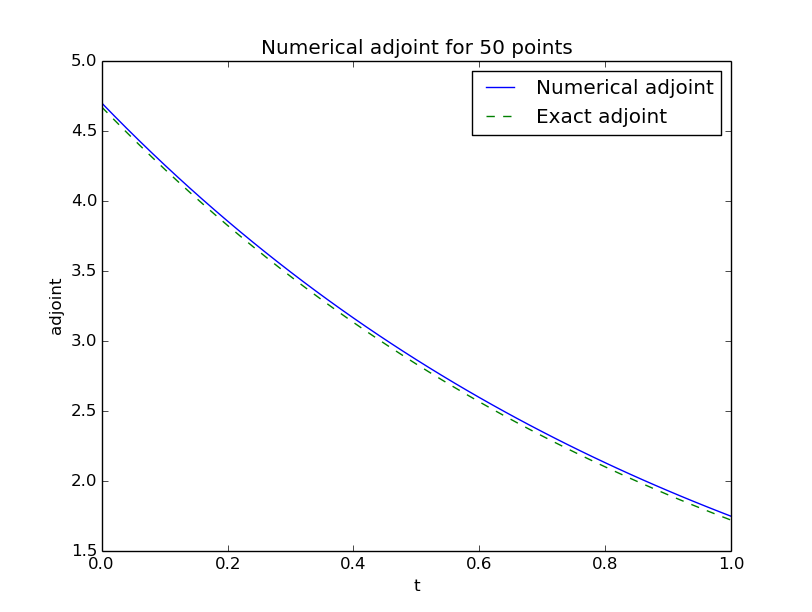
\includegraphics[width=\linewidth]{adjoint_plot.png}
  \caption{Adjoint for $u=0$ and $T=y_T=y_0=\alpha=1$}
  \label{Fig 1}
\end{figure}
\\
\\
\textbf{Testing gradient using finite difference}
\\
Now lets try to test the claims I made earlier about the discrete gradient. I will approximate the gradient using finite difference in the following way:
\begin{align*}
&\hat{J}'(u)^n \approx \frac{\hat{J}(u+\epsilon^n)-\hat{J}(u)}{\epsilon} \\
&\epsilon^n=\epsilon e^n \in \mathbb{R}^{N+1} \ \text{with $\epsilon>0$ small, and $e^n$ the unit vector}
\end{align*} 
As always I let $T=y_T=y_0=\alpha=1$, however this time I choose $u(t)=e^t+t$. I then define the relative error E between the discrete adjoint gradient $\hat{J}'_{\Delta t}(u)$ and the finite difference gradient $\hat{J}'_{\epsilon}(u)$ defined as:
\begin{align*}
E=|\frac{\hat{J}'_{\Delta t}(u)-\hat{J}'_{\epsilon}(u)}{\Delta t}|_{\infty}
\end{align*}
I use this error to test the gradients for different $N$. The result is given in a table below, and I have also added a plot. Note that I as last time calculated convergence rate using least squares, and the result was: $E\leq \Delta tC$, with $C\approx27$.
\begin{center}
    \begin{tabular}{| l | l | l | l | l |}
    \hline
    N & 50 & 100  & 500 & 1000 \\ \hline
    E & 0.5658 &0.2816 &0.0561 & 0.0281	\\ \hline
    \end{tabular}
\end{center}
\begin{figure}
  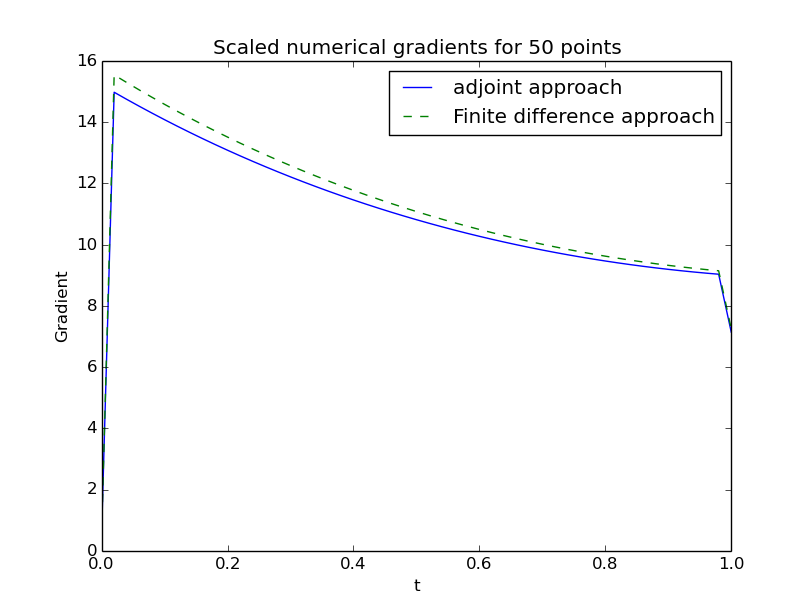
\includegraphics[width=\linewidth]{finite_diff_plot.png}
  \caption{"Relative" gradients for $u=0$ and $T=y_T=y_0=\alpha=1$}
  \label{Fig 2}
\end{figure}
\addcontentsline{toc}{section}{Testing manufactured solution to control problem }
\section*{Testing manufactured solution to control problem}
We now know how to create the gradient of a simple optimal ODE control problem, so we can then try to actually solve the problem using an optimization algorithm. To test if this actually work, lets look at a problem, that has a known non-zero solution. To do this lets tweak the functional that we have used so far in the following way:
\begin{align*}
J(y,u) = \frac{1}{2}\int_0^T(u(t)-1)^2dt + \frac{1}{2}(y(T)-y^T)^2
\end{align*}
This only changes the gradient slightly, since only the $J_u$ term is affected, and now is:
\begin{align*}
\langle J_u(u),s\rangle = \int_0^T (u(t)-1)s(t) dt
\end{align*}
This will then give us the gradient:
\begin{align*}
\langle\hat{J}'(u),s\rangle = \int_0^T(p(t)+u(t)-1)s(t)dt
\end{align*}
Now we want to choose $y^T$ such that $u=1$ yields $J(1)=0$. To do this we notice that the ODE:
\begin{align*}
\left\{
     \begin{array}{lr}
       	y' =  y +1\\
       	   y(0)=y_0
     \end{array}
   \right.
\end{align*}
has the solution $y(t)=(y_0+1)e^t -1$. This means that we should get $J(1)=0$, if we choose $y^T =  (y_0+1)e^T -1$. As above I measure the error between numerical solution $u^N$ and exact solution $u=1$ in max-norm $max_i{|u^N_i-1|}_{i=0}^N$. Then using $T=1$, initial control $u(t)=0$ and the scipy L-bfgs algorithm, I get the following errors:
\begin{center}
    \begin{tabular}{| l | l | l | l | l | l | l |}
    \hline
    N & 500 & 1000  & 1500 & 2000 & 5000 & 8000 \\ \hline
    E & 0.003702 & 0.001844 &0.001227 & 0.000919 & 0.000366 & 0.000228	\\ \hline
    \end{tabular}
\end{center}
Using least squares we get that $E\leq \Delta t^{\alpha}C$, with $C\approx 1.9$ and $\alpha\approx1$. for each $N$, the L-bfgs algorithm used 4 iterations to get to the predefined gradient size tolerance.
\\
\\
Its also interesting to look at what happens when we look at the difference between exact and numeric solution when we are using the penalty method, so below comes result of the same experiment using 2, 4 and 8 partitions of the time interval, and using $\mu=10$ as penalty parameter.
\\
$m=2$:
\begin{figure}
  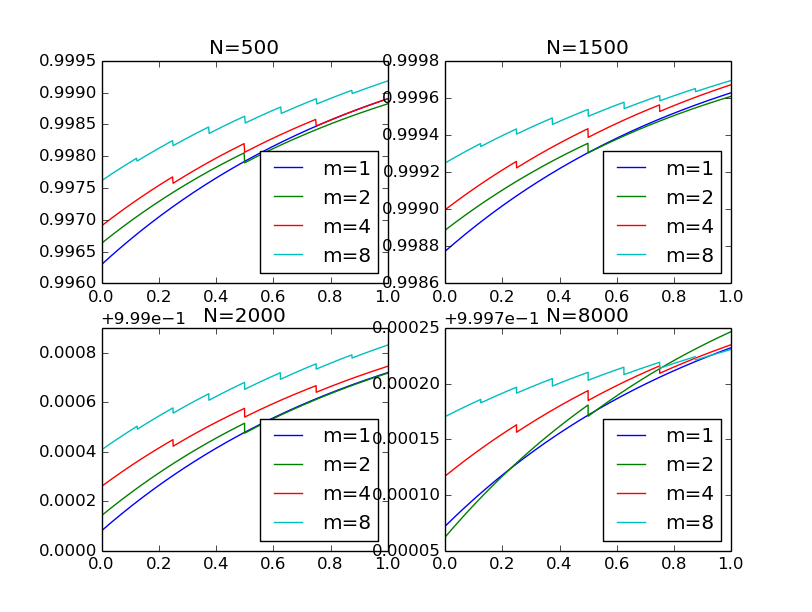
\includegraphics[width=\linewidth]{lin_manu_control.png}
  \caption{The control for different mesh sizes and different number of time interval partitions. }
  \label{Fig 3}
\end{figure}
\begin{center}
    \begin{tabular}{| l | l | l | l | l | l | l |}
    \hline
    N & 500 & 1000  & 1500 & 2000 & 5000 & 8000 \\ \hline
    E & 0.003369 & 0.001675 &0.001113 & 0.000858 & 0.000332 & 0.000238	\\ \hline
    Iter & 14 & 20  & 20 & 14 & 22 & 14 \\ \hline
    \end{tabular}
\end{center}
$m=4$
\begin{center}
    \begin{tabular}{| l | l | l | l | l | l | l |}
    \hline
    N & 500 & 1000  & 1500 & 2000 & 5000 & 8000 \\ \hline
    E & 0.003095 & 0. 001481& 0.001003 & 0.000740 & 0.000303 & 0.000183\\ \hline
    Iter & 40 & 41  & 41 & 43 & 49 & 41 \\ \hline
    \end{tabular}
\end{center}
$m=8$:
\begin{center}
    \begin{tabular}{| l | l | l | l | l | l | l |}
    \hline
    N & 500 & 1000  & 1500 & 2000 & 5000 & 8000 \\ \hline
    E & 0.002385 & 0.001183 &0.000751 & 0.000592 & 0.000246 & 0.000130	\\ \hline
    Iter & 59 & 55  & 69 & 65 & 71 & 73 \\ \hline
    \end{tabular}
\end{center}
As for the non-penalty case i used least square to find the $C\Delta t^{\alpha}$ relation to the error. The following table sums up the results:
\begin{center}
    \begin{tabular}{| l | l | l |}
    \hline
    m & $\alpha$ & C \\ \hline
    2 &0.97 &1.35 \\ \hline
    4 & 1.01&1.63 \\ \hline
    8 & 1.03&1.43 \\ \hline
    \end{tabular}
\end{center}
We notice that the errors and the convergence rate of the penalty solutions are quite similar to the non-penalty approach, however we see that the number of iterations it takes to reach the solution becomes larger as we choose a bigger $m$. 
\\
\\
\textbf{Non-linear ODE}
\\
\\
The ODE equation we have looked at so far is linear and quite simple. To make things more interesting, I will change the equation in the following way:
 \begin{align*}
\left\{
     \begin{array}{lr}
       	y'= F(y) +u\\
       	   y(0)=y_0
     \end{array}
   \right.
\end{align*} 
Here $F:\mathbb{R} \rightarrow \mathbb{R}$, is some differentiable function. We then get $E_y = \frac{\partial}{\partial t} - F'(y)$. To derive the adjoint equation, we need to take the adjoint of the operator $E_y$. This is problematic since it depends on $y$, however since we need to solve the state equation before the adjoint, we can think of $F'(y)$ as a function of $t$. Using this linearisation, we get the following adjoint equation: 
\begin{align*}
\left\{
     \begin{array}{lr}
       	p'(t)=F'(y(t))p(t)\\
       	   p(T)= y(T)-y_T
     \end{array}
   \right.
\end{align*}
The "initial" condition is derived in the usual way assuming: 
\begin{align*}
J(y,u)=L(u) + (y(T)-y_T)^2
\end{align*}
Where $L$ is some functional. When we are dealing with a non-linear ODE, it is more difficult to solve the state equation implicitly. I have therefore only solved this numerically using explicit finite difference for both the state and the adjoint equation. the schemes now look like: 
  \begin{align*}
\frac{y^n-y^{n-1}}{\Delta t} &= F(y^{n-1}) + u^{n-1}\\
y^{n} &= y^{n-1} +F(y^{n-1})+\Delta t u^{n-1} 
\end{align*} 
and for the adjoint equation we get:
\begin{align*}
-\frac{p^n-p^{n-1}}{\Delta t} -F'(y^{n})p^n &=0 \\
p^{n-1} &= (1+\Delta t F'(y^{n}))p^n
\end{align*} 
\\
\\
\textbf{Non-linear example}
\\
\\
Lets look at the case where $F(y) = y^2$, and \begin{align*}
J(y,u) = \frac{1}{2}\int_0^T(u(t)-D)^2dt + \frac{1}{2}(y(T)-y^T)^2
\end{align*}
Want to do a manufactured solution test as did for the  linear ODE case. However since the equation now is non-linear, I don't know its exact solution, when $u$ is non-zero. To get around this I choose $y^T$, by solving the equation numerically with a very high number of unknowns, while I solve the control problem with a smaller number of unknowns. As above I measure the error between numerical solution $u^N$ and exact solution $u=D$ in max-norm $max_i{|u^N_i-1|}_{i=0}^N$. Then using $T=1$, $D=3.1$, initial control $u(t)=0$ and the scipy L-bfgs algorithm, I get the following errors:
\begin{center}
    \begin{tabular}{| l | l | l | l | l | l | l |}
    \hline
    N & 50 & 100  & 150 & 200 & 500 & 1000 \\ \hline
    E & 0.002541 & 0.001222 &0.000779 & 0.000556 & 0.000213 & 0.000083	\\ \hline
    Iter & 6 & 5  & 5 & 5 & 5 & 5 \\ \hline
    \end{tabular}
\end{center}
Using least squares we get that $E\leq \Delta t^{\alpha}C$, with $C\approx 0.22$ and $\alpha\approx1.1$. 
\\
\\
As I did for the linear example, I will look at the difference between exact and numeric solution when we are using the penalty method. Below comes result of the above setting using 2, 4 and 8 partitions of the time interval. As we will see the results when using the penalty method is in this case not as good as for the linear case. To see this clearly I choose $\mu =100$, to really emphasise the penalty term.
\\
$m=2$:
\begin{figure}
  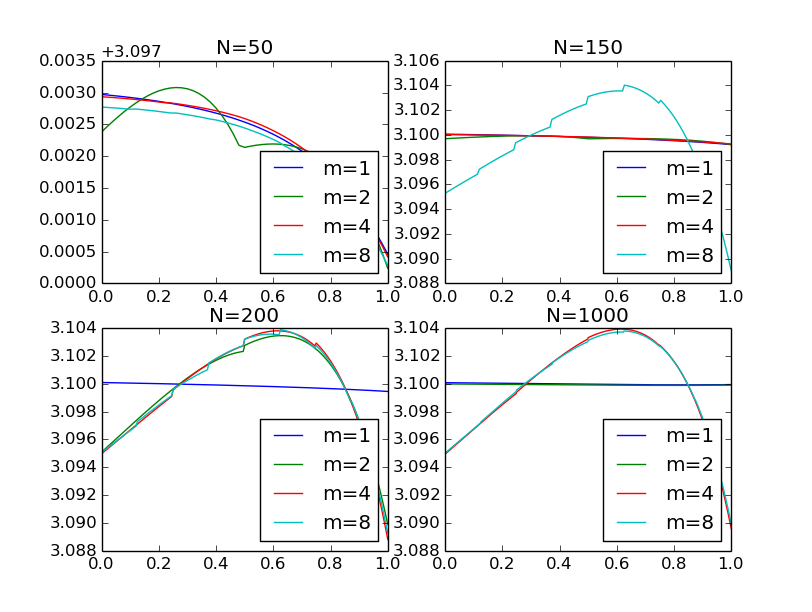
\includegraphics[width=\linewidth]{quad_manu_control.png}
  \caption{The control for different mesh sizes and different number of time interval partitions. We see that for $m=4$ and $m=8$ the control converges to something other than $u=3.1$. However it is still close to $3.2$. We also notice that for $m=2$, we also   get the unnatural solution for some $N$. }
  \label{Fig 4}
\end{figure}
\begin{center}
    \begin{tabular}{| l | l | l | l | l | l | l |}
    \hline
    N & 50 & 100  & 150 & 200 & 500 & 1000 \\ \hline
    E & 0.002763 & 0.001409 &0.000772 & 0.010119 & 0.000263 & 0.000123	\\ \hline
    Iter & 26 & 34  & 49 & 27 & 43 & 48 \\ \hline
    \end{tabular}
\end{center}
$m=4$
\begin{center}
    \begin{tabular}{| l | l | l | l | l | l | l |}
    \hline
    N & 50 & 100  & 150 & 200 & 500 & 1000 \\ \hline
    E & 0.002584 & 0.001605 &0.000723& 0.011186 & 0.010608 & 0.010398\\ \hline
    Iter & 52 & 51  & 53 & 33 & 36 & 40 \\ \hline
    \end{tabular}
\end{center}
$m=8$:
\begin{center}
    \begin{tabular}{| l | l | l | l | l | l | l |}
    \hline
    N & 50 & 100  & 150 & 200 & 500 & 1000 \\ \hline
    E & 0.002718 & 0.001375 &0.010964 & 0.010757 & 0.010096 & 0.010058	\\ \hline
    Iter & 70 & 65  & 59 & 56 & 64 & 57 \\ \hline
    \end{tabular}
\end{center}
From the errors of the $m=4$ and $m=8$ case we see that error does not decrease when deceasing $\Delta t$. We also see this when we use least squares on the error to find a $\Delta t^{\alpha}C$ relation with the error.
\begin{center}
    \begin{tabular}{| l | l | l |}
    \hline
    m & $\alpha$ & C \\ \hline
    2 & 1.04& 0.26\\ \hline
    4 & -0.70& 0.0001\\ \hline
    8 & -0.55&0.0003 \\ \hline
    \end{tabular}
\end{center}
For this example the penalty method produces an answer, that is slightly different from the non penalty method. The reason for this could be that the equation is non-linear.
\\
\\
\textbf{Changing the power of the $y(T)-y^T$ term}
\\
Another way of changing the problem to make it more complex is to alter the functional we have been using so far. I will now look at what happens with the adjoint equation when we change the functional in the following way:
  \begin{align*}
J(y,u) = \int_0^T u^2 dt + \frac{1}{q}(y(T)-y_T)^q
\end{align*}
This change results in a different $J_y$, and therefore a changed adjoint equation. The derivative of $J$ with respect to $y$ is now:
\begin{align*}
J_y = (y(T)-y_T)^{q-1}\delta_T
\end{align*}
This changes the 'initial' condition of the adjoint equation. We now get the following ODE:
\begin{align*}
-\frac{\partial }{\partial t}p(t) &=p(t)  \\
p(T) &= (y(T)-y_T)^{q-1}
\end{align*}
I test this problem with the following parameters:
\begin{align*}
J(y,u) = \int_0^T (u-20)^2 dt + \frac{1}{4}(y(T)-y_T)^4
\end{align*}
this yielded the following table: 
\begin{center}
    \begin{tabular}{| l | l | l | l | l | l | l |}
    \hline
    N & 50 & 100  & 150 & 200 & 500 & 1000 \\ \hline
    E & 0.160164 & 0.038571 &0.014279 & 0.006729 & 0.000438 & 0.000151	\\ \hline
    Iter & 24 & 23  & 23 & 24 & 24 & 24 \\ \hline
    \end{tabular}
\end{center}
Using least squares we get that $E\leq \Delta t^{\alpha}C$, with $C\approx 2533$ and $\alpha\approx2.4$.
\\
\\
As I did for the other examples I will look at the difference between exact and numeric solution when we are using the penalty method. Below comes result of the above setting using 2, 4 and 8 partitions of the time interval, and using $\mu=1$ as penalty parameter.
\\
$m=2$:
\begin{figure}
  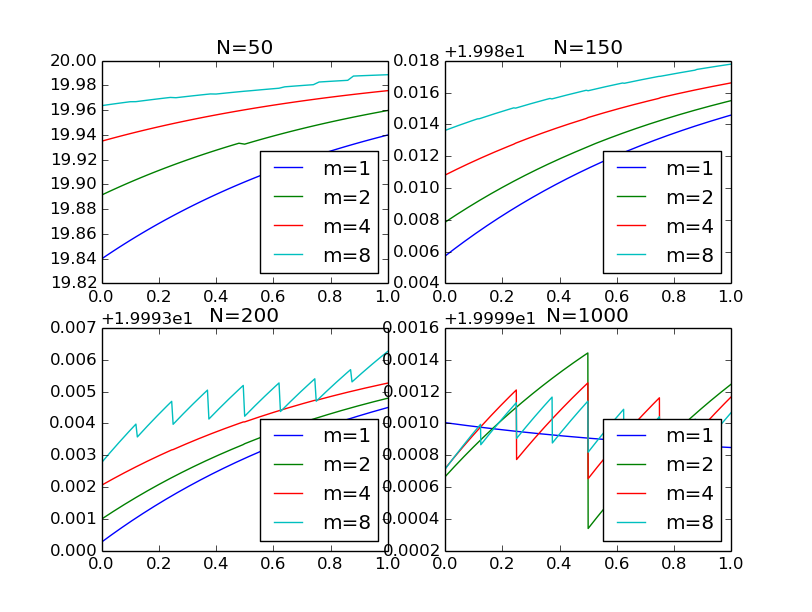
\includegraphics[width=\linewidth]{resC_manu_control.png}
  \caption{The control for different mesh sizes and different number of time interval partitions. }
  \label{Fig 5}
\end{figure}
\begin{center}
    \begin{tabular}{| l | l | l | l | l | l | l |}
    \hline
    N & 50 & 100  & 150 & 200 & 500 & 1000 \\ \hline
    E & 0.108561 & 0.029858 &0.012150 & 0.006006 & 0.000471 & 0.000660	\\ \hline
    Iter & 32 & 46  & 44 & 47 & 49 & 39 \\ \hline
    \end{tabular}
\end{center}
$m=4$
\begin{center}
    \begin{tabular}{| l | l | l | l | l | l | l |}
    \hline
    N & 50 & 100  & 150 & 200 & 500 & 1000 \\ \hline
    E & 0.065024 & 0.020627& 0.009187& 0.004942 & 0.000993 & 0.000347\\ \hline
    Iter & 49 & 51  & 55 & 55 & 51 & 48 \\ \hline
    \end{tabular}
\end{center}
$m=8$:
\begin{center}
    \begin{tabular}{| l | l | l | l | l | l | l |}
    \hline
    N & 50 & 100  & 150 & 200 & 500 & 1000 \\ \hline
    E & 0.036287 & 0.014180 &0.006379 & 0.004230 & 0.000484 & 0.000288	\\ \hline
    Iter & 53 & 56  & 64 & 61 & 78 & 64 \\ \hline
    \end{tabular}
\end{center}
As for the non-penalty case i used least square to find the following $C\Delta t^{\alpha}$ relation to the error. The following table sums up the results:
\begin{center}
    \begin{tabular}{| l | l | l |}
    \hline
    m & $\alpha$ & C \\ \hline
    2 & 1.90& 159.6\\ \hline
    4 & 1.78& 67.2\\ \hline
    8 & 1.73&35.2 \\ \hline
    \end{tabular}
\end{center}
\textbf{Comment on the manufactured solutions}
\\
The manufactured solutions I have used for testing here have showed that both optimization problem is solvable both with and without penalties. There is however one problem with these examples, which i will illustrate by running the linear ODE example with 
\begin{align*}
J(y,u) = \frac{1}{2}\int_0^T(u(t)-1)^2dt + \frac{1}{2}(y(T)-y^T)^2
\end{align*}
using $\mu=0$. This yields the following error tables for different $m$:
\\
$m=2$:
\begin{center}
    \begin{tabular}{| l | l | l | l | l | l | l |}
    \hline
    N & 500 & 1000  & 1500 & 2000 & 5000 & 8000 \\ \hline
    E & 0.000412 & 0.000053 &0.000156 & 0.000114 & 0.000001 & 0.000029	\\ \hline
    Iter & 7 & 7  & 7 & 7 & 6 & 7 \\ \hline
    \end{tabular}
\end{center}
$m=4$
\begin{center}
    \begin{tabular}{| l | l | l | l | l | l | l |}
    \hline
    N & 500 & 1000  & 1500 & 2000 & 5000 & 8000 \\ \hline
    E & 0.000018 & 0.000136& 0.000057& 0.000012 & 0.000030& 0.000009\\ \hline
    Iter & 6 & 7  & 7 & 7 & 7 & 7 \\ \hline
    \end{tabular}
\end{center}
$m=8$:
\begin{center}
    \begin{tabular}{| l | l | l | l | l | l | l |}
    \hline
    N & 500 & 1000  & 1500 & 2000 & 5000 & 8000 \\ \hline
    E & 0.000041 & 0.000090 &0.000049 & 0.000023 & 0.000019 & 0.000010	\\ \hline
    Iter & 6 & 7& 7 & 7 & 7 & 7 \\ \hline
    \end{tabular}
\end{center}
We notice two things here. The first one is that the error is very small, and the second is that the number of iterations to reach this error is very low. This is not what we expect, since the penalty approach should only go to the real solution when $\mu$ goes to infinity. The reason for this anomaly we see by looking closer at the functional 
\begin{align*}
J(y,u) = \frac{1}{2}\int_0^T(u(t)-1)^2dt + \frac{1}{2}(y(T)-y^T)^2
\end{align*}
$J$ is here made up of two parts, the integral over the control \\$f(u)=\frac{1}{2}\int_0^T(u(t)-1)^2dt $, and the difference squared difference \\$g(y)= (y(T)-y^T)^2$. Since we have constructed our problem such that the $u$ that minimize $f$ is also the $u$ that minimizes $g$, minimizing $f$ is equivalent to minimizing $J$. When we set $\mu=0$, we will not be able to solve the adjoint equation on more than the last time interval. However since we still have the $f$ part of the gradient on the entire interval, we still are able to minimize $J$. This means that the examples I have used up until now are not good for understanding how the choice of $\mu$ affects the algorithm.
\addcontentsline{toc}{section}{Relation between $\mu$ and number of time partitions $m$ }
\section*{Relation between $\mu$ and number of time partitions $m$}
Generally one would assume that difference between the numerical solution of the optimization problem with and without penalty would increase when you increase the number of time interval partitions $m$. This seems to be the case as the following example illustrates. Lets solve the following problem:
\begin{align*}
J(y,u) =\frac{1}{2} \int_0^1 (u(t)-100)^2dt + \frac{1}{2}(y(1)-1)^2
\end{align*}  
with 
\begin{align*}
\left\{
     \begin{array}{lr}
       	y' =  y +u\\
       	   y(0)=1
     \end{array}
   \right.
\end{align*}
When solving this numerically I will use $\Delta t= \frac{1}{100}$ and $\mu=20$ for $m=\{1,2,4,8,16\}$ time interval partitions. I then calculate the square integral difference, between the solution of $m=1$ $u_1$and the other cases, i.e.
\begin{align*}
||u_1-u_m||_2^2 = \int_0^1 (u_1(t)-u_m(t))^2dt
\end{align*} 
This yields the following:
\begin{center}
    \begin{tabular}{| l | l |}
    \hline
    m & $ ||u_1-u_m||_2$ \\ \hline
    2 & 2.33\\ \hline
    4 & 6.98\\ \hline
    8 & 15.09\\ \hline
    16 & 24.90 \\ \hline
    \end{tabular}
\end{center}
\begin{figure}
  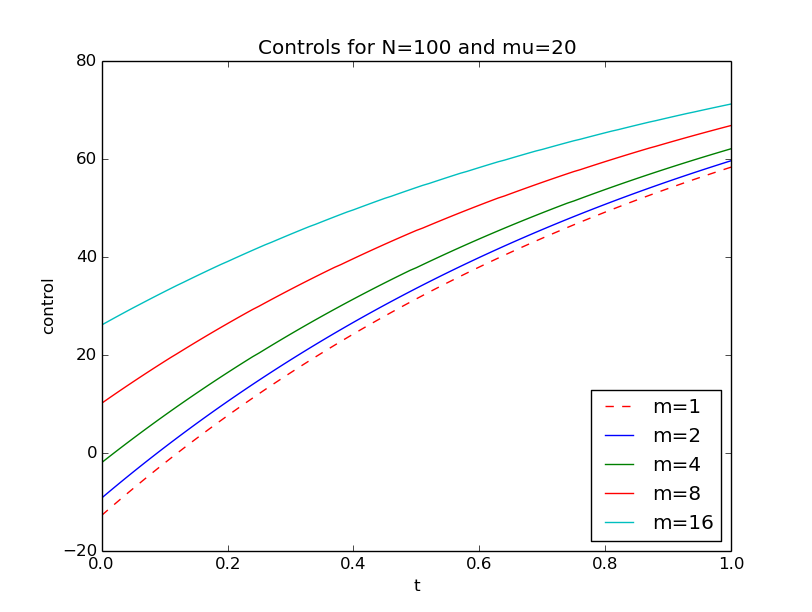
\includegraphics[width=\linewidth]{m_plots.png}
  \caption{Solution of the same problem using different number of time interval partitions.}
  \label{Fig 6}
\end{figure}
We see that increased $m$ increases the difference between the penalty and non-penalty solution. This fact is even clearer observed when looking at the plot of the different controls.
\\
\\
By doing experiments, it seems that the  $||u_1-u_m||_2$ decreases when we increase $N=\frac{1}{\Delta t}$.  If we let the constant $C= \frac{N}{m}$ be fixed, and let $\mu=\beta N$, I will demonstrate that the $||u_1-u_m||_2$ error is similar for increased $m$. For the same problem as above, with $C=50$ and $\beta=0.2$, I got the following:
\begin{center}
    \begin{tabular}{| l | l | l |}
    \hline
    m &  N&$ ||u_1-u_m||_2$ \\ \hline
    2 & 100 &2.33\\ \hline
    4 & 200 &3.73\\ \hline
    8 & 400 &4.46\\ \hline
    16 & 800 &4.84 \\ \hline
    \end{tabular}
\end{center}
\addcontentsline{toc}{section}{Number of lbfgs iterations and lbfgs memory}
\section*{Number of lbfgs iterations and lbfgs memory}
The entire point of parallelizing an algorithm is to decrease its runtime. To check if the penalty method actually achieves a speed-up, I will count the number of iterations the lbfgs algorithm uses to find a solution for both penalty and non-penalty problems. If the number of iterations divided by the number of time interval partitions for a penalty problem is lower than the number of iterations for the non-penalty problem, I will consider this as better performance. What i noticed when testing this is that the number of iterations the lbfgs algorithm needed to do, was related to the length of its memory. This will be demonstrated below: 
\\
\\   
For the experiment I used the linear ODE $y'=y+u$ and the following functional: 
\begin{align*}
J(u,y)=\int_0^T (C_0u(t)-C_1)^2dt + (y(T)-y_T)^2
\end{align*}
This resulted in more iterations for the serial lbfgs. I used different combinations of $C_0$ and $C_1$, to get more results. Results for $C_0=2 $ and $C_1= 1000$ can be found below:
\begin{center}
    \begin{tabular}{| l | l | l |}
    \hline
    m\textbackslash L-BFGS memory & $mem =\max(m,10)$& $mem=3max(m,10)$\\ \hline
    $m=1$  &  5 &  \\ \hline
    $m=2$  &  6 &  6	\\ \hline
    $m=4$ &  8 & 8 \\ \hline
    $m=8$ &  Fail &  12	\\ \hline
    $m=16$ &  Fail & 21 \\ \hline
    $m=32$ &  Fail &  39	\\ \hline
    \end{tabular}
\end{center}
Results for for $C_0=0.1 $ and $C_1= 100$:
\begin{center}
    \begin{tabular}{| l | l | l |}
    \hline
    m\textbackslash L-BFGS memory & $mem =\max(m,10)$& $mem=3max(m,10)$\\ \hline
    $m=1$  &  11 &  \\ \hline
    $m=2$  &  Fail &  12	\\ \hline
    $m=4$ &  Fail & Fail \\ \hline
    $m=8$ &  Fail &  28	\\ \hline
    $m=16$ &  Fail & 35 \\ \hline
    $m=32$ &  Fail &  51	\\ \hline
    \end{tabular}
\end{center}
Results for for $C_0=2 $ and $C_1= -1$:
\begin{center}
    \begin{tabular}{| l | l | l |}
    \hline
    m\textbackslash L-BFGS memory & $mem =\max(m,10)$& $mem=3max(m,10)$\\ \hline
    $m=1$  &  4 &  \\ \hline
    $m=2$  &  5 &  5	\\ \hline
    $m=4$ &  17 & 17 \\ \hline
    $m=8$ &  22 &  20	\\ \hline
    $m=16$ &  51 & 28 \\ \hline
    $m=32$ &  100 &  43	\\ \hline
    \end{tabular}
\end{center}
\textbf{Non-linear example}
\\
To make the problem more difficult we can change the functional by increasing the power of the $y(T)-yT$ term in the following way:
\begin{align*}
J(u,y) = \int_0^T (C_0u(t)-C_1)^2dt + \frac{1}{4}(y(T)-y_T)^4
\end{align*}
When doing this one need to change the adjoint equation, but it is quite simple. Here is a result of solving this problem using $C_0=1 $ and $C_1= 0.5$:
\begin{center}
    \begin{tabular}{| l | l | l |}
    \hline
    m\textbackslash L-BFGS memory & $mem =\max(m,10)$& $mem=3max(m,10)$\\ \hline
    $m=1$  &  14 &  \\ \hline
    $m=2$  &  16 & 21 	\\ \hline
    $m=4$ &  22 & 21 \\ \hline
    $m=8$ &  Fail &  28	\\ \hline
    $m=16$ &  Fail & 28 \\ \hline
    $m=32$ &  124 &  52	\\ \hline
    \end{tabular}
\end{center}
\begin{figure}
  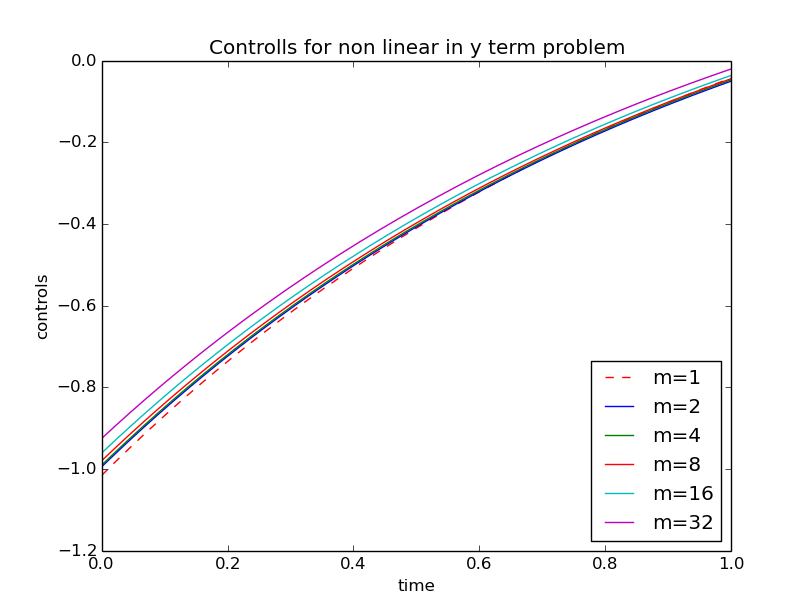
\includegraphics[width=\linewidth]{non_linY.png}
  \caption{Plot of control for different m values, that are the result of the non-linear problem I have iteration results for below. }
  \label{Fig 7}
\end{figure}
\newpage
\section{Burgers Equation}
Lets look at the optimal control with PDE constraint problem, where the equation is the burgers equation:
\begin{align*}
u_t + uu_x - \nu u_{xx} &= 0 \ \text{for $(x,t)\in \Omega\times(0,T)$}\\
u(x,t) &= h(x,t) \ \text{for $(x,t) \in\partial\Omega\times(0,T)$ } \\
u(x,0) &= g(x) \ \text{for $x \in\Omega$ }
\end{align*} 
Here $\Omega = (a,b)$. The functional is on the form:
\begin{align*}
J(u(g),g) = \int_0^T\int_{\Omega} u(x,t)^2 dxdt
\end{align*}
Here we want to minimize $J$ with respect to the initial condition $g$. If we differentiate $J$ with respect to $g$, we get:
\begin{align*}
\hat{J}'(g)(s) &= \langle u'(g)^*J_u,s \rangle \\
&= \langle -E_gp,s \rangle
\end{align*}
where $p$ is the solution of the adjoint equation:
\begin{align*}
E_u^*p = J_u
\end{align*}
By $E$ I mean burgers equation, which means that:
\begin{align*}
E_u &= \frac{\partial}{\partial t} + u_x + u\frac{\partial}{\partial x} - \nu\Delta + \delta_{t=0} + \delta_{\partial \Omega} \\
E_g &= -\delta_{t=0} \\
E_u^* &= -\frac{\partial}{\partial t}  -u\frac{\partial}{\partial x}- \nu\Delta + \delta_{t=T} + (1+h)\delta_{\partial \Omega} \\
J_u &= 2u
\end{align*}
The adjoint equation would then look like:
\begin{align*}
-p_t -up_x - \nu p_{xx} &= 2u \ \text{for $(x,t)\in \Omega\times(0,\infty)$}\\
p(x,t) &= 0 \ \text{for $(x,t) \in\partial\Omega\times(0,\infty)$ } \\
p(x,T) &= 0 \ \text{for $x \in\Omega$ }
\end{align*}
This would mean that the gradient of $\hat{J}$ is:
\begin{align*}
\hat{J}'(g)(s) = \langle p(\cdot,0), s\rangle
\end{align*}
\textbf{m time intervals}
\\
Divide $[0,T]$ into $m$ intervals $[T_{i-1},T_i]$, where $0=T_0<T_1<\cdots<T_m=T$. We then solve burgers equation for $\{u^i(x)\}_{i=1}^m$ on each interval with initial conditions $\{\lambda_i(x)\}_{i=0}^{m-1}$, where $\lambda_0(x)=g(x)$. As for the two interval case, we need to add penalty terms to the functional, to solve the optimization problem. The penalized functional looks like this:
\begin{align*}
J(u(g),g,\lambda) = \int_0^T\int_{\Omega} u(x,t)^2 dxdt + \frac{\mu}{2}\sum_{i=1}^{m-1}\int_{\Omega} (u^i(x,T_i)-\lambda_i(x))^2dx
\end{align*}
The state equation on each interval looks like:
\begin{align*}
u_t^i + u^iu_x^i - \nu u_{xx}^i &= 0 \ \text{for $(x,t)\in \Omega\times(T_{i-1},T_i)$}\\
u^i(x,t) &= h(x,t) \ \text{for $(x,t) \in\partial\Omega\times(T_{i-1},T_i)$ } \\
u^i(x,0) &= \lambda_{i-1}(x) \ \text{for $x \in\Omega$ }
\end{align*} 
If write this equation as en operator $E^i$, we get:
\begin{align*}
E^i &= u_t^i + u^iu_x^i - \nu u_{xx}^i +\delta_{t=T_{i-1}}(u^i-\lambda_{i-1}) + \delta_{\partial \Omega}(u^i-h)
\end{align*}
Now lets look at the gradient. The gradient expression for $m$ intervals depends on both $g$ and $\lambda$, which is now a vector $\lambda =(\lambda_1,...,\lambda_{m-1})$. First the gradient:
\begin{align*}
\langle \hat{J}'(g,\lambda), (s,l)\rangle =\langle -(E_g+E_{\lambda})p , (s,l)\rangle + \langle J_g+J_{\lambda}, (s,l)\rangle
\end{align*}
Again $p$ is the solutions of the adjoint equations $(E_u^i)^*p^i = J_{u^i}$. Lets state the values of the different components in the gradient: 
\begin{align*}
E_u^i&=\frac{\partial}{\partial t} + u_x^i + u^i\frac{\partial}{\partial x} - \nu\Delta + \delta_{t=T_{i-1}} + \delta_{\partial \Omega} \\
E_g^1 &= -\delta_{t=0} \\
E_{\lambda_i}^i &= -\delta_{t=T_i} \ i\neq 1 \\
J_g &= 0 \\
J_{u} &= 2u + \mu\sum_{i=1}^{m-1} (u^i - \lambda_i)\delta_{t=T_i} \\
\langle J_{\lambda_i},l\rangle &= -\mu\int_{\Omega} (u^i(x,T_i)-\lambda_i(x))l_i(x)dx
\end{align*}
This gives us the following adjoint equations:
\begin{align*}
-p_t^i -u^ip_x^i - \nu p_{xx}^i &= 2u^i \ \text{for $(x,t)\in \Omega\times(T_{i-1},T_i)$}\\
p^i(x,t) &= 0 \ \text{for $(x,t) \in\partial\Omega\times(T_{i-1},T_i)$ } \\
p^m(x,T) &= 0 \ \text{for $x \in\Omega$ } \\
p^i(x,T_i) &= \mu(u^i(x,T_i)-\lambda_i(x)) \ \text{for $x \in\Omega$ and $i\neq m$}
\end{align*}
We can also show that the gradient looks like the following:
\begin{align*}
\langle \hat{J}'(g,\lambda), (s,l)\rangle &=\langle -(E_g+E_{\lambda})p , (s,l)\rangle + \langle J_g+J_{\lambda}, (s,l)\rangle \\
&= \int_{\Omega} p^1(x,0)s(x)dx + \sum_{i=1}^{m-1}\int_{\Omega} (p^{i+1}(x,T_i)-p^i(x,T_i))l_i(x)dx
\end{align*}
\section{Extra stuff}
I will add some things that I have done, that I don't think is that relevant, or that turned out to not work.
\addcontentsline{toc}{section}{Augmented Lagrange}
\section*{Augmented Lagrange}
An alternative to the penalty method is the augmented Lagrange method. This method is similar to the penalty method, but it is apparently more stable. The main difference is in the functional, which now reads as:
\begin{align*}
J(y,u,\lambda) &= \int_0^T u^2 dt + \frac{1}{2}(y_n(T)-y_T)^2 + \frac{\mu}{2} \sum_{i=1}^n (y_{i-1}(T_i)-\lambda_i)^2 + \sum_{i=1}^n \Gamma_i(y_{i-1}(T_i)-\lambda_i) \\
&= \int_0^T u^2 dt + \frac{1}{2}(y_n(T)-y_T)^2 +  (y_{i-1}(T_i)-\lambda_i)\sum_{i=1}^n (\Gamma_i+\frac{\mu}{2}(y_{i-1}(T_i)-\lambda_i))
\end{align*}
The difference is that we add non squared penalty terms with a Lagrange multiplication factor $\Gamma_i$. Since we change the functional, its derivative changes, however the only the $J_y$ and $J_{\lambda_i}$ terms change:
\begin{align*}
J_{\lambda_i}&= -\mu(y_{i-1}(T_i)-\lambda_i) -\Gamma_i\\
J_y &= \delta_{T_{n+1}}(y_n(T_{n+1})-y_T) +  \sum_{i=1}^n \delta_{T_{i}}[\mu(y_{i-1}(T_i)-\lambda_i ) + \Gamma_i]
\end{align*}
This changes both the adjoint equations and the gradient. For the adjoint equations the change happens in the 'initial' condition:
\begin{align*}
-\frac{\partial }{\partial t}p_i &=p_i  \\
p_i(T_{i+1}) &= \mu(y_{i}(T_{i+1})-\lambda_{i+1} ) + \Gamma_{i+1}
\end{align*}
For the gradient the change happens in the $\lambda$ part of the control:
\begin{align*}
\langle \hat{J}'(u,\lambda), (s,l)\rangle&=\langle -(E_u+E_{\lambda})p, (s,l)\rangle + \langle J_u+J_{\lambda}, (s,l)\rangle \\
&= \int_0^T (u+p)s \ dt +\sum_{i=1}^n[(p_{i}(T_i) -p_{i-1}(T_i) )- \Gamma_i]l_i
\end{align*}
The $\Gamma$ need to be updated for each iteration, i.e. each time we change $\mu$.
\newpage
\addcontentsline{toc}{section}{Comments on LBFGS and special Hessian update technique }
\section*{Comments on LBFGS and special Hessian update technique}
\textbf{General algorithm}
\\
The BFGS and L-BFGS are quasi-Newton methods for solving unconstrained optimization problems on the form:
\begin{align*}
\min_{x \in \mathbb{R}^n} J(x)
\end{align*} 
This can be looked on as solving the system of equations on the form \\$\nabla J(x) = F(x)=0$. Using the Newton method, that can be derived using Taylor series, we get the following iteration for solving the system:
\begin{align*}
x^{k+1} = x^k - F'(x^k)^{-1}F(x^k)
\end{align*}
Here $x^k \in \mathbb{R}^n$, $F:\mathbb{R}^n \rightarrow \mathbb{R}^n$ and $F':\mathbb{R}^{n\times n} \rightarrow \mathbb{R}^{n\times n}$. $F'$ is also the Hessian of $J$. The difference between Newton and BFGS is that we in BFGS approximate $F'(x)^{-1}$ with a matrix that we for each iteration update with information gained form current information. This means that we get a series of matrices $\{H^k\}$, that hopefully approximates the real hessian $H^kx^k \approx F'(x^k)^{-1}$. Without going into detail lets state the update formula for $H^k$:
\begin{align*}
H^{k+1} &= (\mathbb{I} - \frac{s_k {y_k}^T}{\rho_k})H^k(\mathbb{I} - \frac{s_k {y_k}^T}{\rho_k}) + \frac{s_k {s_k}^T}{\rho_k} \ \text{ where} \\
s_k &= x^{k+1} - x^k \\
y_k &= \nabla J(x^{k+1}) - \nabla J(x^k) \\
\rho_k &= s_k^Ty_k
\end{align*} 
We also need an initial approximation $H^0$ to the inverted hessian. This is typically set to be $H^0 = \beta\mathbb{I}$, where $\mathbb{I}$ is the identity matrix and $\beta$ is some constant. The BFGS algorithm at step $k$ then looks like:
\begin{align*}
&\text{1. update control by:} \ x^{k+1}= x^{k} - H^kF(x^{k}) \\
&\text{2. update $s_k$, $y_k$ and $\rho_k$ as described above} \\
&\text{3. update $H$ by:} \ H^{k+1} = (\mathbb{I} - \frac{s_k {y_k}^T}{\rho_k})H^k(\mathbb{I} - \frac{s_k {y_k}^T}{\rho_k}) + \frac{s_k {s_k}^T}{\rho_k}
\end{align*}
\textbf{L-BFGS}
\\
The difference between BFGS and L-BFGS is that one, in the L-BFGS case, base the approximation of the inverted Hessian on only the latest iterations. The size of the memory can wary. 
\\
\\
\textbf{Optimal control with ODE constraints}
\\
We want to solve an optimal control problem with ODE constraints in parallel  using the penalty approach. The problem looks as follows:
\begin{align*}
\min_{u} J(y(u),u) &= \frac{1}{2}(\int_0^T u^2 dt + (y(T)-y_T)^2) \\
y'(t) &= ay(t) +u(t) \\
y(0) &=y_0
\end{align*} 
For the penalty approach we partition the time domain $[0,T]$ into $m+1$ intervals $\{[T_i,T_{i+1}]\}_{i=0}^m$, and solve the problem on each interval separately. To enforce continuity we add penalty terms to the $J$ functional. This leads to a new functional:
\begin{align*}
J(y,u,\lambda) = \int_0^T u^2 dt + \frac{1}{2}(y_n(T)-y_T)^2 + \frac{\mu}{2} \sum_{i=1}^n (y_{i-1}(T_i)-\lambda_i)^2
\end{align*}
Here $y_i$ is the solution of the ODE restricted to interval $i$, and $\lambda = \{ \lambda_i\}_{i=1}^n$ are the initial values of $y_i$. Using the adjoint equations $p_i$, we get the following gradient for $J$ with respect to $u$ and $\lambda$:
\begin{align*}
\langle \hat{J}'(u,\lambda), (s,l)\rangle&=\int_0^T (u+p)s \ dt +\sum_{i=1}^n(p_{i}(T_i) -p_{i-1}(T_i) )l_i \\
&= \int_0^T (u+p)s \ dt +\sum_{i=1}^n(p_{i}(T_i) -\mu(y_{i-1}(T_i)-\lambda_i) )l_i
\end{align*} 
If we discritize the time interval using $N$ points, we get the following control:
\begin{align*}
x = (u^1,...,u^N, \lambda_1, ...,\lambda_m)
\end{align*}
and the gradient:
\begin{align*}
\nabla J(x) &= (\Delta t (u^1+p^1),\Delta t (u^2+p^2),...,\Delta t (u^N+p^N),p_{1}(T_1) -p_{0}(0),..,p_{m}(T_m) -p_{m-1}(T_m)) \\
&=(\Delta t (u^1+p^1),...,\Delta t (u^N+p^N),p_{1}(T_1) -\mu(y_{0}(T_1)-\lambda_1),..,p_{m}(T_m) -\mu(y_{m-1}(T_m)-\lambda_m)) \\
&= (\Delta t\{u^j+p^j\}_{j=1}^N|p_i(T_i)) + \mu(\{0\}_{j=1}^N|\lambda_i - y_{i-1}(T_i))
\end{align*}
This expression for the gradient motivates a special initial Hessian approximation technique, where one for each $\mu$ iteration remember the Hessian, and then passes it on to the next iteration. We then use the previous Hessian with updated $\mu$ as initial Hessian $H_0$ instead of the identity.
\\
\\
\textbf{Testing Hessian approximation technique} 
\\
For testing I solve the problem:
\begin{align*}
\min_{u} J(y(u),u) &= \frac{1}{2}(\int_0^1 u^2 dt + (y(1)-1)^2) \\
y'(t) &= y(t) +u(t) \\
y(0) &=1
\end{align*}
Numerically I solve the state equation and the adjoint equation using backward Euler method, and the trapezoidal rule for integration. I solved this problem without partitioning and penalties and with partition and penalty using both normal L-BFGS and L-BFGS with the $\mu$-trick. I partition the domain $I=[0,1]$ into ten uniform parts and use $N=2000$ and $N=3000$ points to discretize $I$. To measure the performance of the two penalty methods, I counted the number of iterations needed in the L-BFGS algorithm to reach the wanted tolerance. For both dizcritizations I used $\mu=0.1N$ and $\mu=0.5N$. I got the following results: 
\begin{figure}
  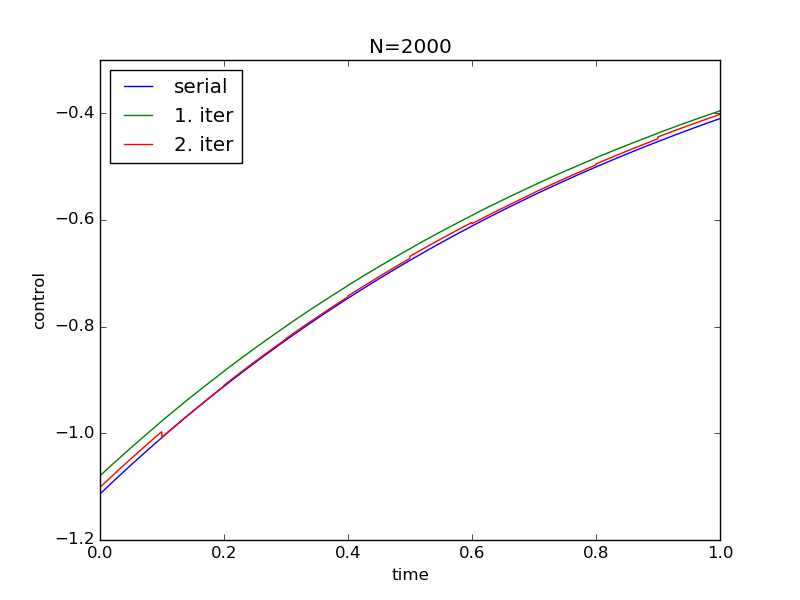
\includegraphics[width=\linewidth]{mufail2000.png}
  \caption{The second iteration gives a solution closer to the non-penalty solution, as we would expect. However the control from the second iteration is less smooth than the control from the first iteration.}
  \label{Fig 8}
\end{figure}
\begin{center}
    \begin{tabular}{| l | l | l |}
    \hline
     & iterations L-BFGS & iterations  L-BFGS + $\mu$-trick \\ \hline
    $N=2000$ and $\mu=0.1N$ &  15 & 15 \\ \hline
    $N=2000$ and $\mu=0.5N$&  16 &  28	\\ \hline
    $N=3000$ and $\mu=0.1N$ &  15 & 15 \\ \hline
    $N=3000$ and $\mu=0.5N$&  27 &  28	\\ \hline
    \end{tabular}
\end{center}
I also added a plot of the controls I get from solving the problem using the $\mu$-trick compared with the control we get from not using any penalties. What both the iteration count and plot tells us is that the $\mu$-trick is not working very well. The number of iterations using is either the same or bigger than what we see for not using old Hessian. From the plot we also see that the solutions gets less smooth and distorted when using the $\mu$-trick. I have also done other tests, and they all yield similar results.
\addcontentsline{toc}{section}{References}
\bibliography{maday}
\bibliographystyle{plain}

\end{document}
